\chapter{Обзор предлагаемого решения} \label{ch3}

Данная глава посвящена обзору предлагаемого решения, описания его реализации.
Перед разбором деталей, стоит дополнительно рассмотреть 
потенциальный инструментарий лаборатории, который необходимо подключить к MAS.

Как показывает практика, язык программирования Python является одним из самых популярных
языков программирования: для лабораторных исследовательских процессов - это не исключение.
Используемые инструменты, будь то внутренние реализованные алгоритмы или специфические 
сторонние библиотеки, реализованы, как правило, именно на этом языке.

Потому перечисленные выше способы вызова функций LLM-агентами охватывают 
большинство инструментов, с которыми могут работать исследователи: 
для инструментов, реализованных на языке программирования Python, 
можно использовать JSON-вызовы или возможности кодогенерации. На \firef{fig:ch3:tools} 
указано отображение инструментов лабораторий с интерфейсами,
через которые они могут быть подключены к MAS для автоматизации решения задач.

\begin{figure}
    \center
	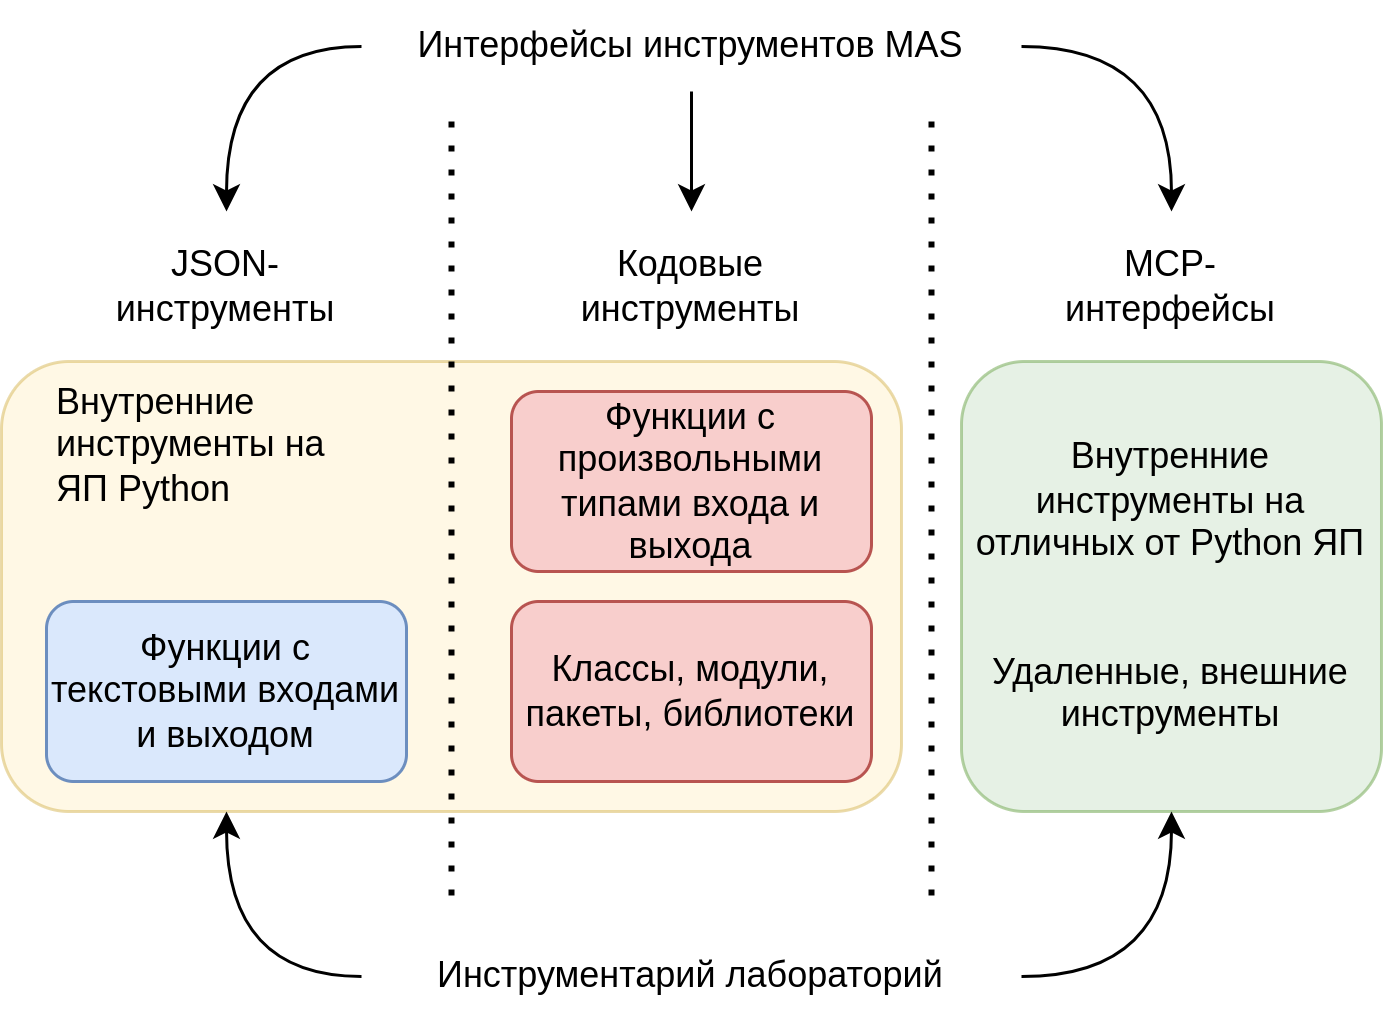
\includegraphics[scale=0.24]{sources/tools_interfaces.drawio.png}
	\caption{Соответствие между используемыми интерфейсами MAS и инструментами лабораторий.} 
	\label{fig:ch3:tools}  
\end{figure}

Остальные, редкие, но возможные отличные сценарии использования 
решаются путем редуцирования их к перечисленным в обзоре литературы
способов вызова инструментов: так, например, в случае, если существует 
удаленный инструментарий, работающий через запросы или написанный на отличном языке 
программирования, достаточно воспользоваться MCP-интерфейсом 
для создания MCP-сервера и подключения к предлагаемой MAS.

Теперь рассмотрим, как реализовывалось решение, работающее с указанным набором 
средств подключения инструментов. 

\section{ExCodeAgent-MM: агент кодогенерации.} \label{ch3:sec1}

Для работы с кодовыми инструментами можно оттолкнуться от решения,
предлагаемого в работе \cite{codeact}, только модифицировав его для того, чтоб агент 
кодогенерации, помимо непосредственной генерации и запуска кода, обладал 
еще двумя следующими свойствами:
\begin{enumerate}
    \item работал с вариативным числом инструментов;
    \item поддерживал работу с мультимодальными данными и их анализ;
\end{enumerate} 

\begin{figure}
    \center
	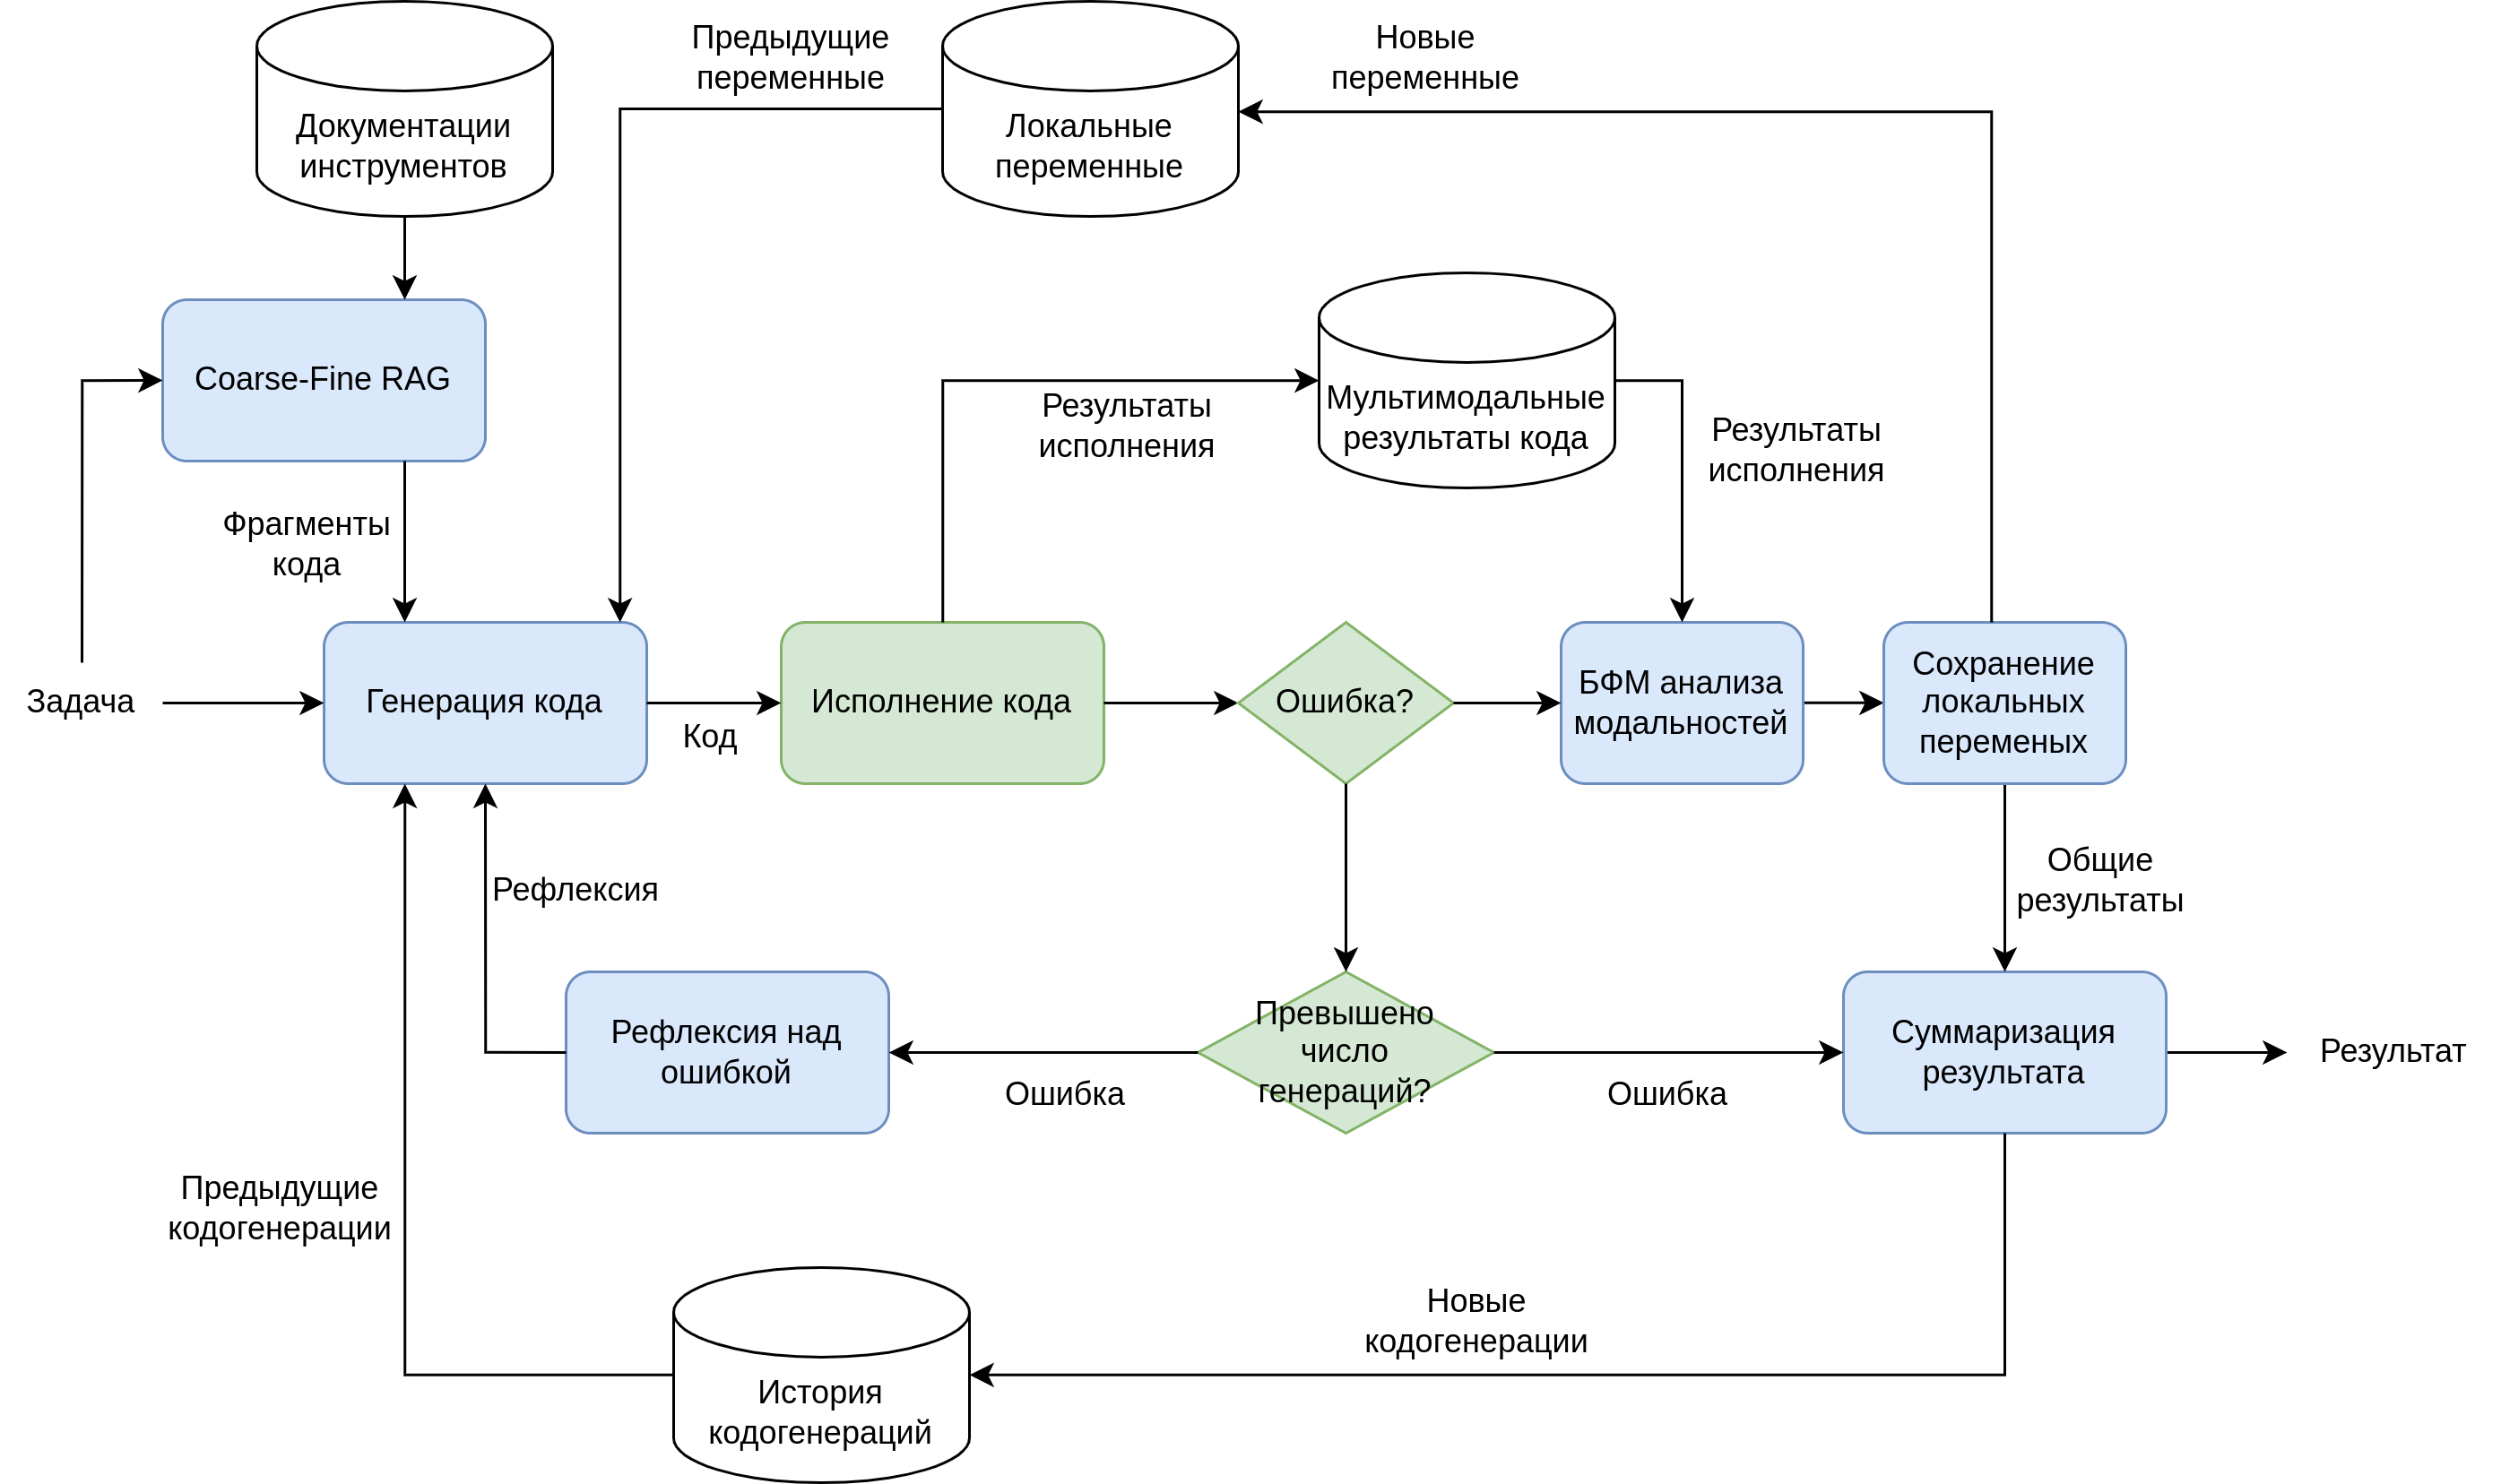
\includegraphics[scale=0.15]{sources/диаграмма агента кодогенерации.drawio.png}
	\caption{Общая структура агента кодогенерации.} 
	\label{fig:ch3:excodeagent-mm}  
\end{figure}

С этими целями был построен агент кодогенерации, изображенный на \firef{fig:ch3:excodeagent-mm}. 
Принципы, по которому он устроен, подробно расписаны в секциях далее.

\subsection{Coarse-Fine RAG: интеграция кодовых инструментов.} \label{ch3:sec1:subsec1}

Для генерации кода с вариативными функциями, классами, модулями и библиотеками необходимо, 
как было рассказано ранее, не только добавлять информацию об этих элементах в контекст 
модели, но и делать это \textit{эффективно}. 
Остановимся пока на том, как можно структурировать информацию.

\begin{figure}
    \center
	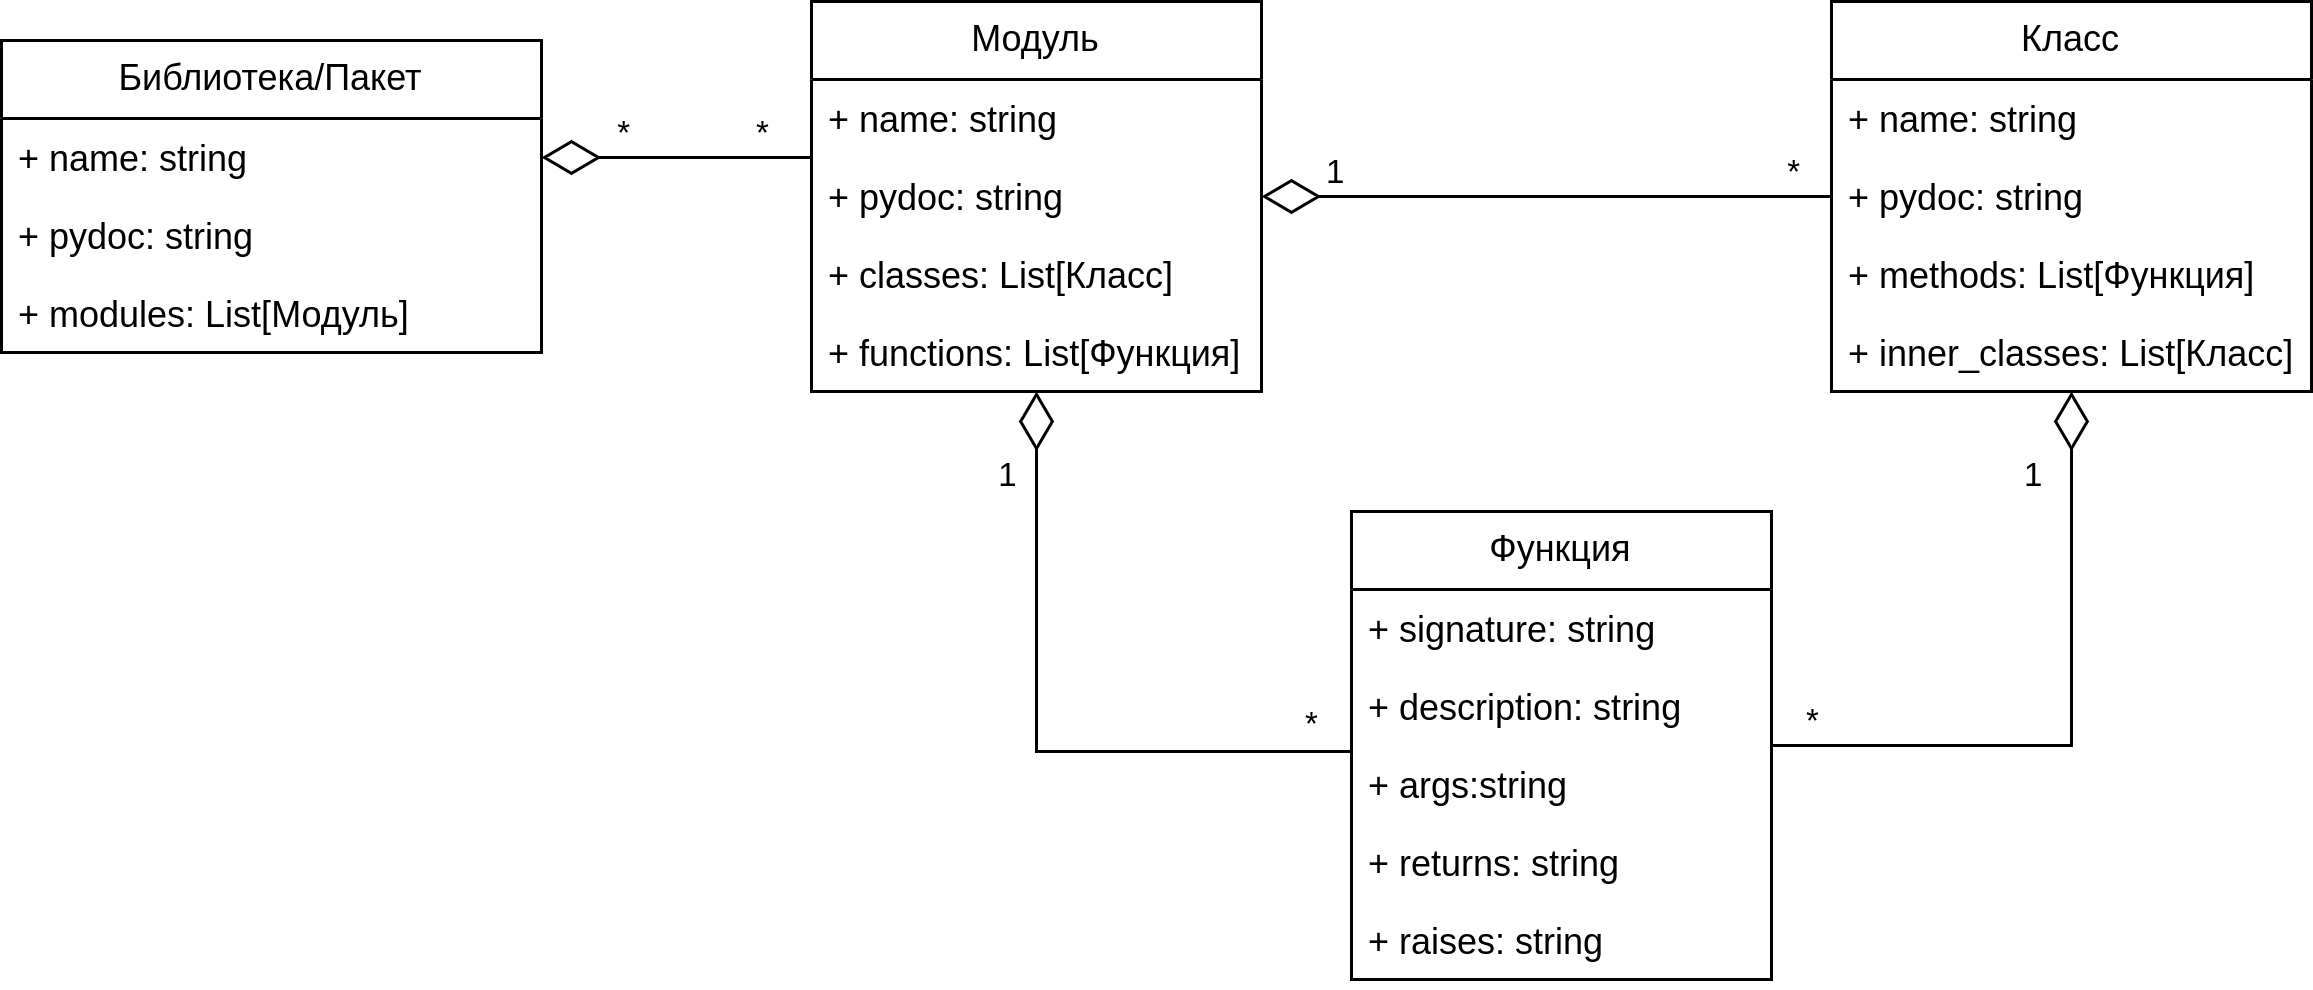
\includegraphics[scale=0.16]{sources/документирование pydoc.drawio.png}
	\caption{Диаграмма классов. Вложенность элементов кодовых инструментов
 и форма их документирования.} 
	\label{fig:ch3:code_tools}  
\end{figure}

На \firef{fig:ch3:code_tools} представлена информация, как в общем виде
структурируются пакеты, модули, классы, методы, как они относятся друг к другу,
а также как они документируются. 
Как видно, у каждого элемента есть свое описание, притом у функций и методов - 
оно самое подробное. 
Самое примечательное, что это описание не требуется в каком-то 
специализированном для данного проекта формате или в отдельном документе - 
это обычные pydoc строки, которые используются для документирования и автодокументирования
кода: они доступны у элементов посредством обращения к полю ``.\_\_doc\_\_'' и имеют 
общепризнанные стандарты \cite{google_pydoc}. 
Это свойство Python - чрезвычайно важно для формаировании информации об
иструментах и её передачи в контекст LLM-модели для последующей генерации.

Процедура извлечения документации из кода и её структурирование происходит 
по принципу обхода элементов библиотек, модулей и классов в глубину: 
действительно, все эти элементы имеют строение дерева,
по которому можно пройтись и для каждого элемента-узла сконструировать его документацию.
После обхода, вся считанная документация сохраняется в упрощенной структуре, указанной
на \firef{fig:ch3:pydocs}: имя и краткая документация задаются пользователями вручную, а полная
структурированная документация в лице списка классов и функций - извлекается автоматически. 

\begin{figure}
    \center
	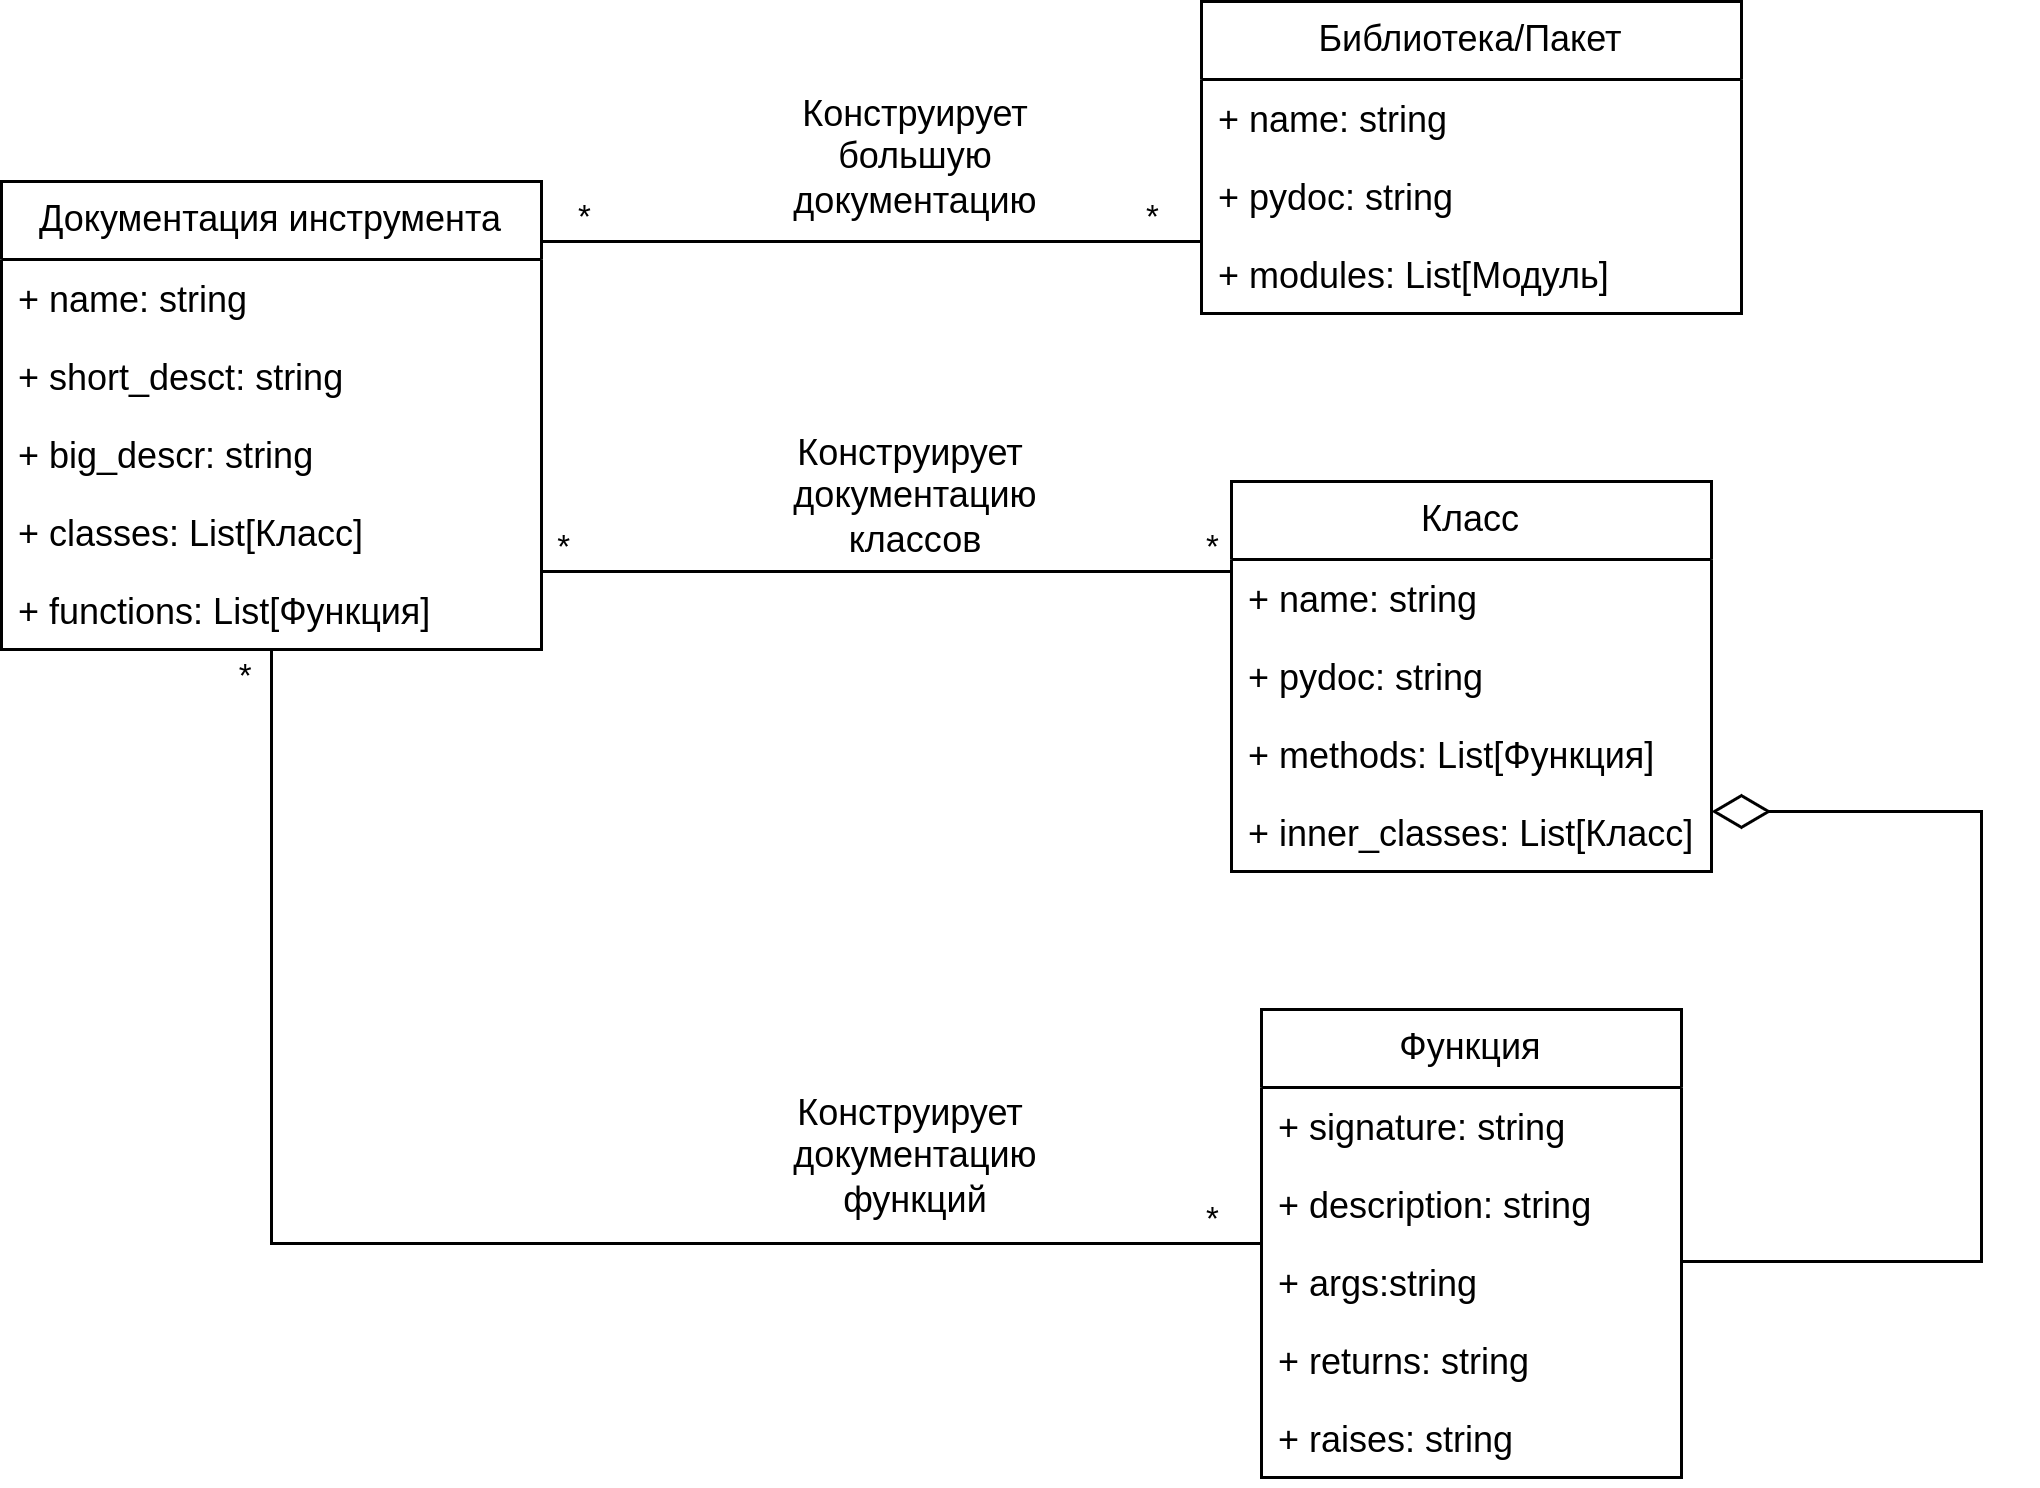
\includegraphics[scale=0.16]{sources/генерация документации.drawio.png}
	\caption{Диаграмма классов из класса-документации и классов, её формирующую.} 
	\label{fig:ch3:pydocs}  
\end{figure}

После того, как документации всех переданных инструментов 
были загружены, необходимо передавать её в контекст LLM
для генерации кода. Есть два варианта, как это можно сделать:
\begin{itemize}
    \item загружать целиком всю документацию о всех инструментах в контекст в LLM вместе;
    \item выборочно подавать фрагменты документаций для последующей кодогенерации.
\end{itemize}

Первый вариант в условиях неограниченности ресурсов кажется выигрышным, однако LLM обладают
спецификой ``путаться'' в выборе различных методов и классов, число которых, 
как правило, может быть очень большим даже при малом количестве переданных библиотек. 
Кроме того, не стоит и забывать, что ресурсы всё же ограничены, 
а модели имеют квадратичную сложность от длины контекста. 
Второй вариант при правильном выборе фрагментов документаций нивилирует эти проблемы: потому
далее будет рассмотрен разработанный эффективный метод подгрузки фрагментов 
документации для кодогенераций. Он также продемонстрирован на \footnote{рис}.

Извлечение полезных фрагментов документаций в предлагаемом решении происходит 
в два этапа путём двойной фильтрации информации об инструментах:
\begin{enumerate}
    \item \textit{Грубая (``coarse'') фильтрация}: LLM на основе внутренних рассуждений 
и кратких пользовательских описаний инструментов выбирает, какие именно из инструментов 
будут актуальны для решения задач. 
По выбранным инструментам создается ``грубая'' документация -
документация инструмента без подробного описания функций в виде аргументов, возвращаемых 
типов и исключений: только их краткое описание и сигнатура.  
    \item \textit{Точная (``fine'') фильтрация}: ``Грубые'' документации выбранных 
инструментов подгружается вновь в LLM для выбора нужных функций и методов для решения задачи. 
Выбранные функции используются для обогащения ``грубой'' документации подробной информацией
об этих функций для последующей кодогенерации.
\end{itemize}

Такой процесс ``coarse-fine'' фильтрации можно рассматривать как двойное модифицированное
использование HyDE, где используются такие же предположения и рассуждения модели: 
модификация в данном конкретном случае заключается в использовании структурированности 
данных в документации.

Стоит отметить, что попытки применения классических методов выбора 
фрагментов при помощи RAG на основе косинусной близости вместро предложенного
алгоритмы могут оказаться малоэффективным: 
методы на основе косинусной близости работают только с векторными представлениями 
фрагментов и не учитывают то, \textit{как структурированны} эти фрагменты и 
\textit{что} описано во фрагменте в явном виде.

Теперь перейдем к вопросу учета и анализа мультимодальных данных.

\subsection{Анализ мультимодльных данных} \label{ch3:sec1:subsec3}

Оригинальная система CodeAct предлагает единственный способ анализа мультимодальных данных:
только посредством вывода информации о данных в поток вывода.
Предлагаемое решение позволяет анализировать мультимодальные двумя способами:
\begin{itemize}
    \item посредством текстовой информации в потоке вывода, полученной при исполнении кода;
    \item посредством использования БФМ для анализа дополнительных модальностей. 
\end{itemize}

На фоне роста числа как общих БФМ (например, для анализа инфографиков), так и 
специализированных БФМ \cite{alphafold3}, а также невозможности описать данные 
одними только аналитическими метриками, дополнительная возможность исследовать 
данные является скорее полезной, чем избыточной.

Эта возможность достигается за счет реализации трех элементов:
\begin{itemize}
    \item подключения БФМ для анализа дополнительной модальности;
    \item создания callback-функции, которая захватывает данные из сгенерированного и 
сохраняет их;
    \item описания этой самой callback-функции, а также других дополнительных инструкций
в системном промпте для кодогенерации. 
\end{itemize} 

Общий принцип анализа дополнительных модальностей таков: LLM-агент кодогенерации генерирует 
код, в котором согласно прописанным инструкциям используются callback-функции с передачей
данных специальной модальности в качетве аргумента. При вызове callback-функции происходит
копирование данных специальной модальности для последующей передачи БФМ модели. В случае
успешного выполнения всего сгенерируемого кода - описание входной задачи, текстовый выход
в потоке вывода, а также скопированные данные специальной модальности отправляются 
на вход БФМ для генерации текстового описания данных. 

% Реализация анализа каждой модальности происходит путем реализации интерфейса классом.
% Пример реализации инструкций и класса для захвата инфографиков, генерируемых при помощи
% библиотеки ``matplotlib'' представлена в Приложении № \footnote{добавить аппендикс}.

\subsection{Генерация, выполнение и валидация кода} \label{ch3:sec1:subsec2}

Генерация кода для выполнения задачи происходит с учетом переданных из 
Coarse-Fine RAG фрагментов необходимой документации, а также переданных пользователем
списке рекомендованных популярных библиотек (например, ``numpy'' или ``matplotlib'').

Исполнение сгенерированного кода происходит в несколько этапов:
\begin{itemize}
    \item \textit{проверка импортирования модулей}: посредством отдельного исполнения строк кода 
со словами ``import'' и ``from'' происходит проверка досягаемости используемых 
кодовых инструментов, а также заранее рекомендованных библиотек и фреймворков. В случае 
ошибки возращается соответствующая ошибка для рефлексии и выборе других библиотек;
    \item \textit{исполнение кода}: при помощи функции ``exec(code, locals)'' с передачей
сгенерированного кода и ранее полученных при предыдущем исполнении локальных переменных 
происходит выполнение нового кода;
    \item \textit{повторная генерация кода}: происходит в случае ошибки при исполнении. LLM 
передается задача, необходимые фргменты документации, последняя попытка кодогенерации с 
рассуждениями, а также ошибка при исполнении - всё это с инструкцией ``обдумать'' 
ошубику и попытаться выявить её причину. После рефлексии - происходит повторная генерация; 
Результат рефлексии вместе со всем перечисленным выше подается в качестве входа
для повторной кодогенерации с целью исправить ошибку;
    \item \textit{сохранение локальных переменных и результатов кода в специальные 
переменные-хранилища}: в сучае успешной генерации кода новые переменные и 
мультимодальные результаты сохраняются для последующего использования. 
\end{itemize}

Выделение специальных хранилищ необходимо по двум причинам:
\begin{itemize}
    \item \textit{последовательность задач кодогенерации}: 
поскольку задачи для кодогенерации направлены на решение общей главной задачи
и все они поступают друг за другом, для решения вновь пришедшего задания
необходимо учитывать контекст решения предыдуших;
    \item \text{переиспользование разных модальностей}: помимо анализа модальностей
полученные результаты используются в других целях - в выводе в 
графическом интерфейсе и в формировании Jupyter Notebook'ов со сгенерированными командами
и сохраненными результатами выводом. 
\end{itemize}

Генерация Jupyter Notebook'ов с сгенерированными кодами и результатами исполнения
в формате изображений и текста в поток вывода - разработанная в рамках задачи опция, 
позволяющая переиспользовать сгенерированный код для решения типовых задач, а также
формирования графических документов для анализа данных. 

\section{ExCodeAct: конечная мультиагентная система для различных инструментов.} \label{ch3:sec2}

С целью создать рефлексирующую и рассуждающую модель для работы не только с кодовыми 
инструментами лаборатории, но и с прочими другими указанными на \firef{fig:ch3:tools},
было создана сеть, сочетающая оригинальное решение ReAct с разработанным агентом
кодогенерации ExCodeAgent-MM, а также MCP инструментами. Изображение разработанной системы,
названной ExCodeAct, представлено на \firef{fig:ch3:excodeact}.

\begin{figure}
    \center
	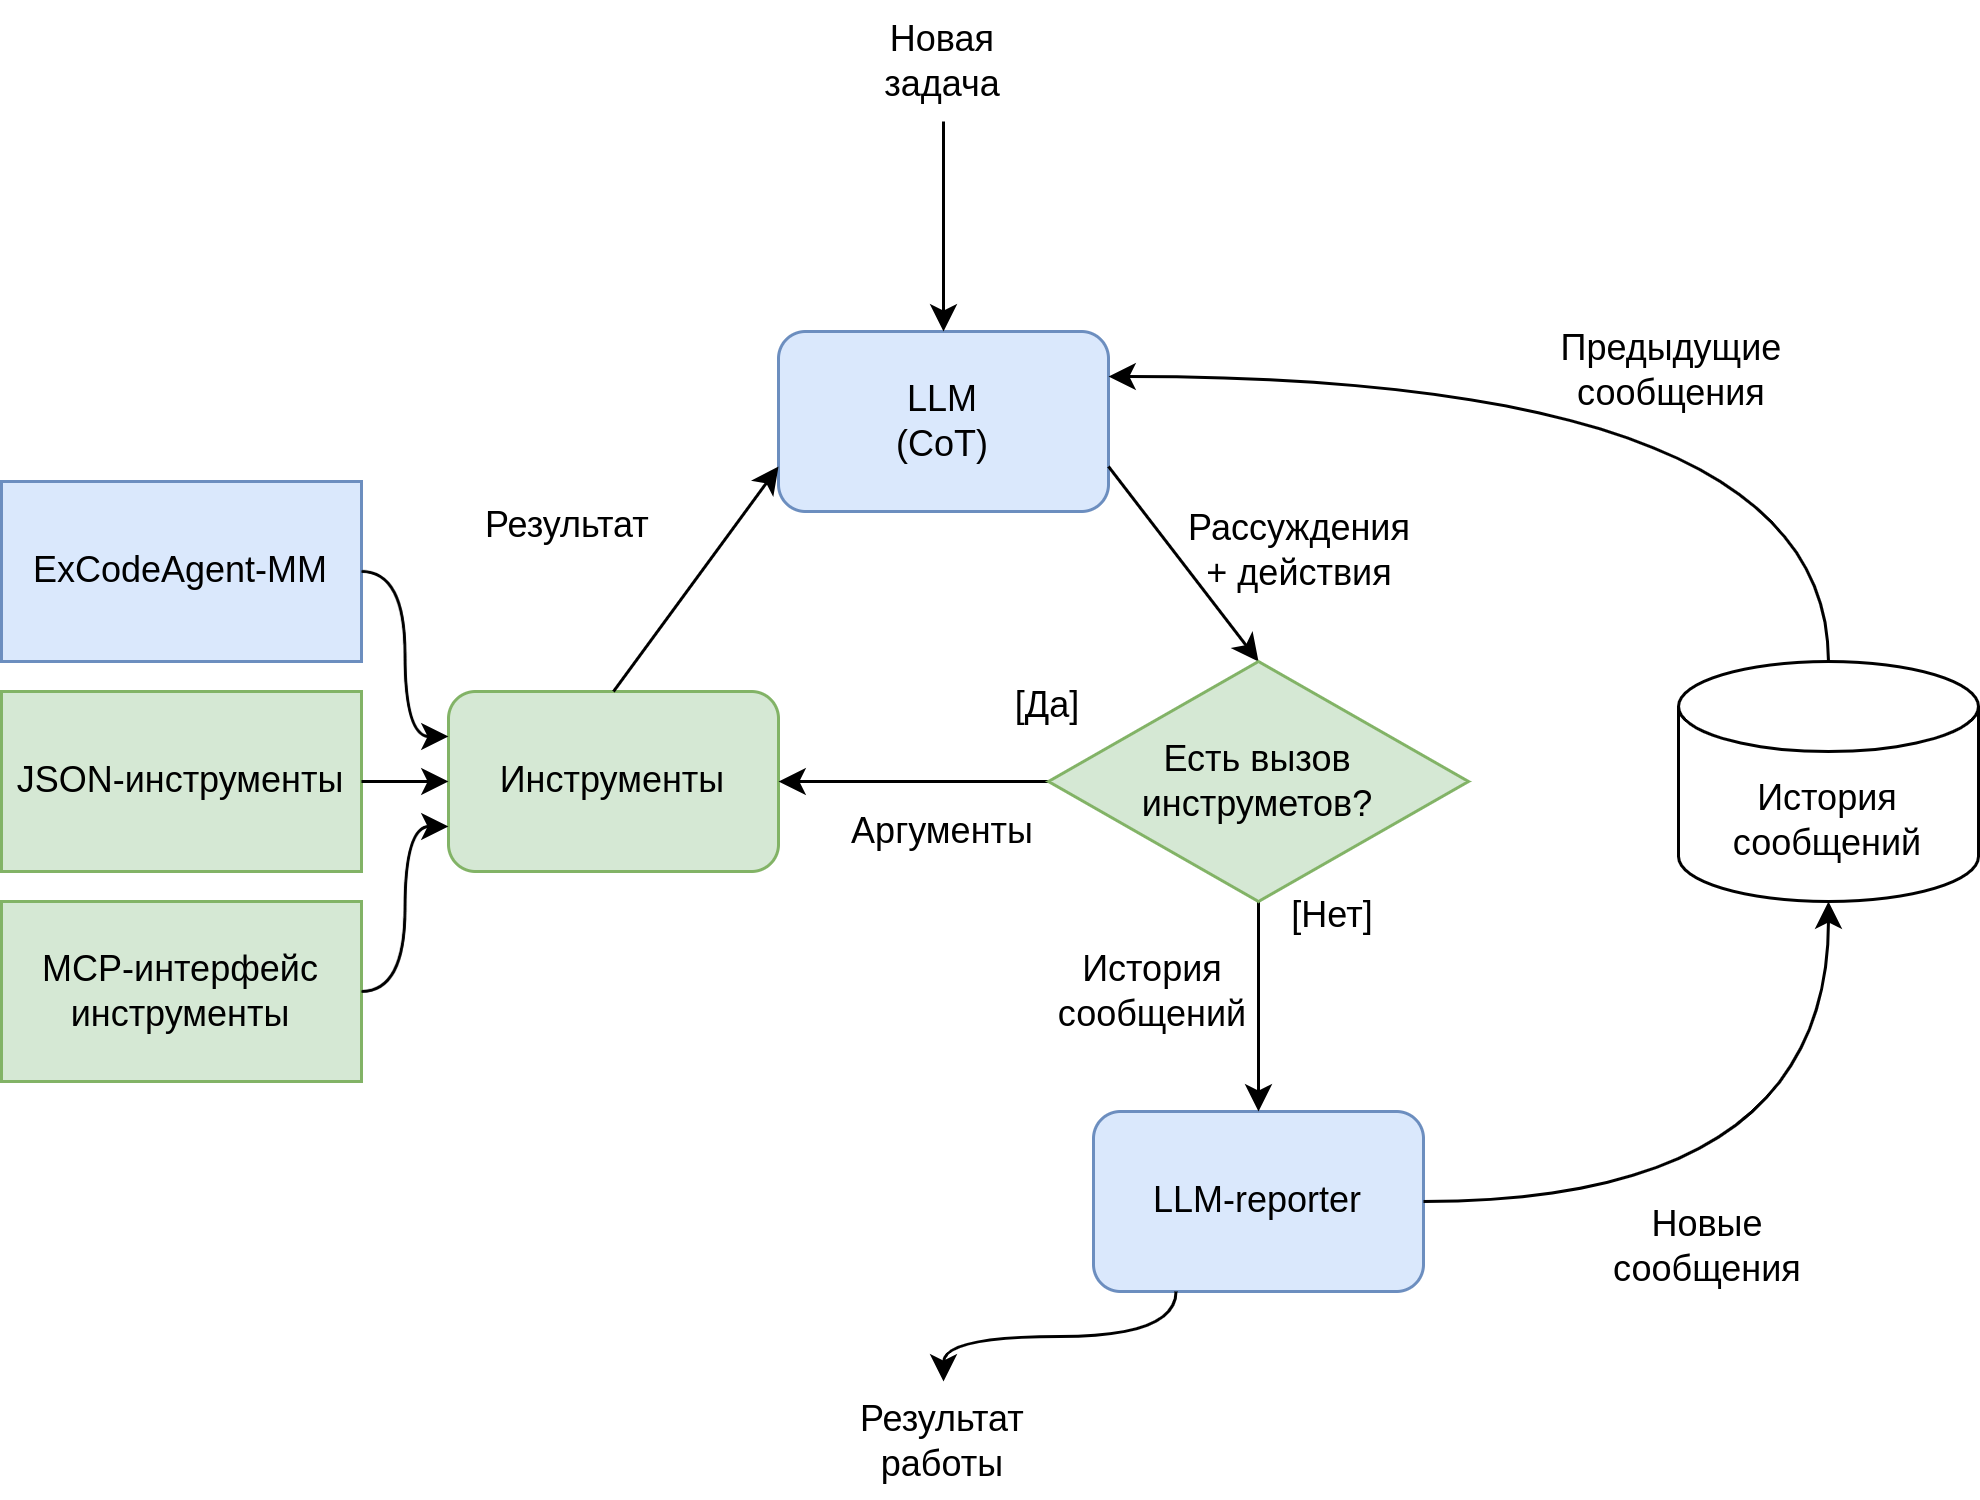
\includegraphics[scale=0.24]{sources/ExCodeAct-MM.png}
	\caption{Структура полной мультиагентной системы ExCodeAct.} 
	\label{fig:ch3:excodeact}  
\end{figure}

Предлагаемая система циклично ``рассуждает'' над выбором инструментов для решения подзадач,
вызывает инструменты, а затем оценивает результаты и выбирает новые инструменты.

Данная структура выбрана неспроста: система ReAct способна не только автоматизировать 
исполнение тривиальных рутинных задачи, она обеспечивая гибкость в используемых инструментах,
которые вызываются через узел ``Инструменты'', что увеличивает спектр решаемых задач. 
Кроме того, данная система естественно встраивается в формат диалога
с пользователем, который может дополнительно передавать новые задачи, 
связанные с предыдущими. 
Заключительной причиной в выборе базовой системы для модификации послужил тренд
в развитии качества рассуждений больших языковых моделей, 
что позволит в будущем решать более сложные задачи куда менее усложненными системами.

Используемые данные об инструментах, будь то кодовые инструменты или MCP-интерфейсы с 
JSON-инструментами, ровно как и системные инструкции к различным агентам сети,
задаются в файле конфигурации в формате YAML - формат имеет низкий порог к требуемым знаниям
 для заполнения исследователями.

Все специальные хранилища, которые используются в процессе работы, являются простыми 
переменными: хранилища для сообщений - списки, хранилище для переменных - 
словарь (хэш-таблица), где ключами служат названия переменных, а 
хранилище для pydoc документаций - словарь, в котором ключами служат имена кодовых 
инструментов.

\section{Детали реализации} \label{ch3:sec3}

Предлагаемое решение было реализовано при помощи фреймворков разработки мультиагентных
систем на базе LLM LangChain и LangGraph Для тестирования различных вариаций систем и выбора конечного решения использовался
среда LangSmith \cite{langchain, langgraph, langsmith}.

Графический интерфейс предлагаемого решения реализован при помощи фреймворка Streamlit,
предлагающего возмножность быстро и удобно разворачивать LLM-агентов и MAS, 
работающих на базе LangGraph \cite{streamlit}.

% Тут пишется уже просто про особенности реализации, фреймворки, как все управляется и тд и тп.
